% IMPORTANT! In order for the document to compile, one needs to use XeLaTeX or LuaLaTeX as compiler. This can be done in  Overleaf by Menu -> Settings -> Compiler -> Choose XeLaTeX/LuaLaTeX
\documentclass[t,24pt,aspectratio=169]{beamer}

\usepackage{hyperref}
\usepackage{listings}
\usepackage{KUstyle}
\usepackage{cite}
\usepackage{graphicx}
\usepackage{tikz}
\usetikzlibrary{arrows.meta, positioning}
\graphicspath{ {./Week2gr/} }

\toplinje{Text at top} % The text at top. Remove the command if no text is desired

\begin{document}

% The first slide. One can, for instance change the main title, the subtitle, speaker, KU-unit and date
{
\setbeamertemplate{background}{
\includegraphics[width=\paperwidth,height=\paperheight]{KU/forside.pdf}}
\begin{frame}
    \begin{textblock*}{\textwidth}(0\textwidth,0.1\textheight)
        \begin{beamercolorbox}[wd=7.8cm,ht=7.3cm,sep=0.5cm]{hvidbox}
            \fontsize{5}{10}\fontfamily{ptm}\selectfont \textls[200]{UNIVERSITY OF COPENHAGEN}
            \noindent\textcolor{KUrod}{\rule{6.8cm}{0.4pt}}
        \end{beamercolorbox}
    \end{textblock*}
    \begin{textblock*}{\textwidth}(0\textwidth,0.1\textheight)
        \begin{beamercolorbox}[wd=7.8cm,sep=0.5cm]{hvidbox}
                \Huge \textcolor{KUrod}{Week 3 - progress}
                \vspace{0.5cm}
                \par
                \Large Project in Causal Discovery
                \vspace{0.5cm}
                \par
                \normalsize Daryna Nedilko
                
                \today
        \end{beamercolorbox}
    \end{textblock*}
    \begin{textblock}{1}(6.3,11.38)
        
\includegraphics[width=1cm]{KU/KU-logo.png}
    \end{textblock}
\end{frame}
}

% A standard slide. It's important that [hoved] is included after \begin{frame}
\begin{frame}[hoved]
\frametitle{What did I do this week?}
\begin{itemize}
    \item read some papers
    \item read more papers
    \item almost gave up on my ideas
    \item played with Python
    \item browsed the internet
\end{itemize}
\end{frame}

\begin{frame}[hoved]
\frametitle{My initial idea was...}
... to work with text data and LLMs(vague, right?). However:
\begin{itemize}
    \item hard to understand how to represent text data for the task
    \item The research is very recent
    \item Focus mostly on LLM insights rather then sentiment - does not smoothly alighn with causal discovery
    \item requires too much work and research for a 6-week project
    \item but I don't give up yet!
\end{itemize}
\end{frame}

\begin{frame}[hoved]
\frametitle{The papers I have read}
\begin{itemize}
    \item LLMS for Causality
    \begin{itemize}
        \item Causal graph discovery using LLMs \cite{jiralerspong2024efficientcausalgraphdiscovery}
        \item CAUSALDANN: Estimating Causal Effects from Text Using LLMs 
        \cite{guo2025estimatingcausaleffectstext}
        \item and an array of observational papers
    \end{itemize}
    \item Causal Discovery Algorithms
    \begin{itemize}
        \item Caught up on the algorithms presented by my colleagues at the last meeting
    \end{itemize}
\end{itemize}
\end{frame}


\begin{frame}[hoved]
\frametitle{Causal Discovery with LLMS\cite{jiralerspong2024efficientcausalgraphdiscovery}}
\begin{itemize}
    \item No observational data is needed
    \item Uses Breadth-First Search (BFS) to construct causal graphs(outputs DAG)
    \item  Only a linear number of LLM queries are needed to build the DAG
    \item Human-like approach(semantic reasoning) to guess the connection between two variables based on metadata 
\end{itemize}
\end{frame}

\begin{frame}[hoved]
\frametitle{Causal Discovery with LLMS\cite{jiralerspong2024efficientcausalgraphdiscovery} : A diagram}
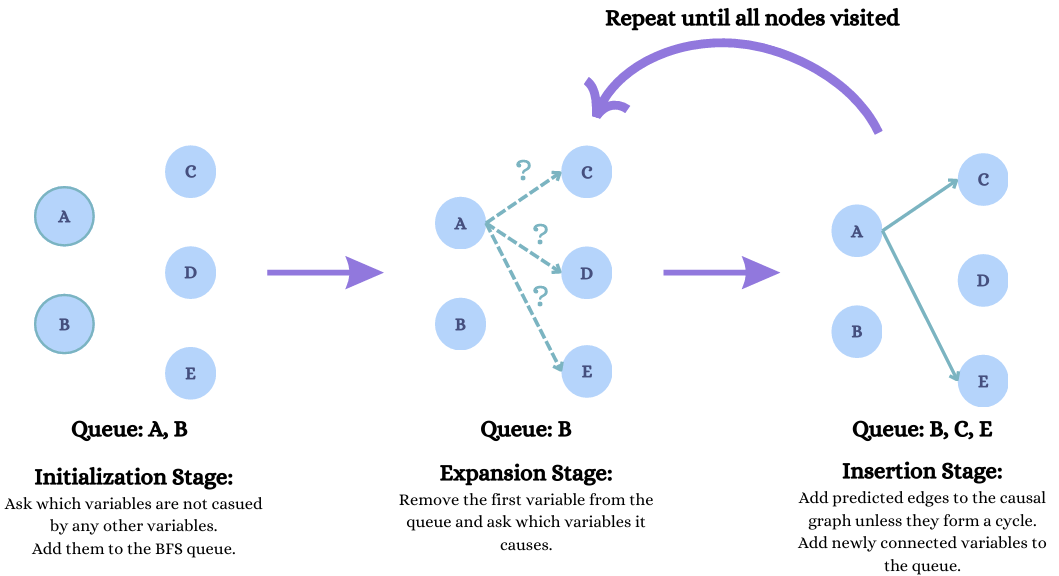
\includegraphics[scale = 0.55]{Presentations/Week2gr/Causality w LLMs.png}
\end{frame}

\begin{frame}[hoved]
\frametitle{CAUSALDANN: Estimating Causal Effects from Text Using LLMs \cite{guo2025estimatingcausaleffectstext}}
% \begin{columns}
%     \begin{column}{0.4\textwidth}
        \begin{itemize}
            \item NOT A CAUSAL DISCOVERY PAPER, but it doesn't make it less interesting
            \item The aim is to estimate the effect of the treatment T on the outcome Y, accounting for confounding and/or non-confounding covariates - does it for 3 cases(hybrid datasets/various tasks)
            \item Works within the potential outcomes framework
            \item Using LLMS to formulate text interventions
            \item Predicts unobserved outcomes of text interventions
            \item Uses domain adaptation to mitigate domain shift between observed and unobserved data
            \item  Applying this approach to causal estimation on real data requires the assumption that LLMs can \textbf{reliably } infer unobserved data points through text transformation based on observed human behaviour - we cannot be sure about that.
        \end{itemize}
%     \end{column}
%     \begin{column}{0.3\textwidth}
%         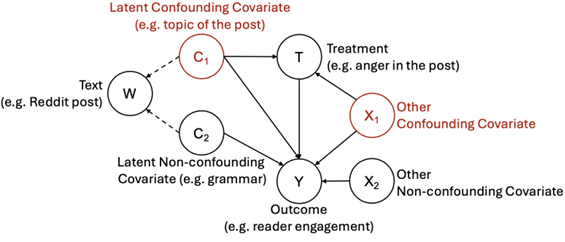
\includegraphics[width=\textwidth]{Presentations/Week2gr/Знімок екрана 2025-05-12 194146.png}
%     \end{column}
% \end{columns}
\end{frame}

\begin{frame}[hoved]
\frametitle{CAUSALDANN: Estimating Causal Effects from Text Using LLMs \cite{guo2025estimatingcausaleffectstext}}
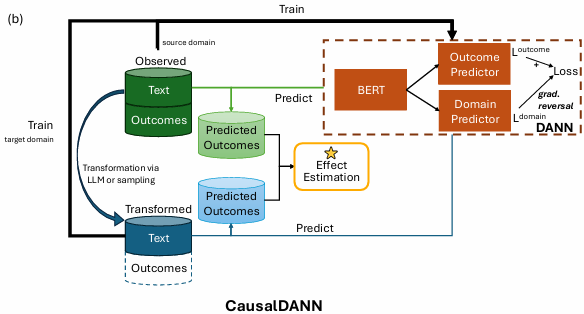
\includegraphics{Presentations/Week2gr/DANN.png}
\end{frame}

\begin{frame}[hoved]
\frametitle{Python}
\begin{itemize}
\item Packages I could start, and I will cover
\begin{itemize}
    \item \textbf{\href{https://causal-learn.readthedocs.io/en/latest/index.html}{causal-learn }}
    \item \textbf{gCastle}
\end{itemize}
\item Packages that make me sad, as it didn't go well on the installation stage(LMK if you succeed in starting any of them)
    \begin{itemize}
    \item \textbf{CausalDiscoveryToolbox (CDT)}: Supports constraint-based (PC, GES), score-based (CAM), and functional approaches (ANM, LiNGAM, IGCI, NOTEARS).
    
    \item \textbf{DoWhy}: Focuses on causal inference via the potential outcomes framework; supports four steps: model, identify, estimate, refute.

    \item \textbf{NOTEARS}: Optimization-based approach; supports linear and nonlinear causal discovery via continuous DAG constraints.

    \item \textbf{Lingam}: Linear non-Gaussian acyclic models; supports DirectLiNGAM, ICA-LiNGAM, and other variants.

    \item \textbf{py-causal (Tetrad via Python)}: Wrappers for Tetrad’s Java-based methods; supports PC, FCI, GES, GFCI, LiNGAM, and more.

    \end{itemize}
\end{itemize}
\end{frame}


\begin{frame}[fragile]
\frametitle{causal-learn}

\begin{columns}
    % Left column: Text
    \begin{column}{0.5\textwidth}
        \begin{itemize}
            \item CI Tests: Fisher-z (incl. missing), Chi-Square, Kernel-based (KCI), G-Square
            \item Constraint-based: PC, FCI, CD-NOD (PC with unobserved changing factors)
            \item Score-based: GES, Exact Search (A*, Dynamic Programming)
            \item LiNGAM-based and permutation-based methods
            \item Output: (CP)DAG or adjacency matrix(LiNGAM)
        \end{itemize}
    \end{column}

    % Right column: Code
    \begin{column}{0.5\textwidth}
        \lstset{
          language=Python,
          basicstyle=\ttfamily\small,
          keywordstyle=\color{blue}\bfseries,
          commentstyle=\color{gray},
          stringstyle=\color{red},
          showstringspaces=false,
          frame=single,
          breaklines=true
        }

        \begin{lstlisting}
from causallearn.search.ConstraintBased.PC import pc
from causallearn.utils.GraphUtils import GraphUtils
#"chisq" - crashed memory loss, "kci" - crashed too long execution
graph = pc(data, indep_test = "fisherz", alpha=0.05)
GraphUtils.to_pydot(
    graph.G, labels= <YOUR_LABELS>
).write_png("<YOUR_NAME>.png")

            
        \end{lstlisting}
    \end{column}
\end{columns}

\end{frame}

\begin{frame}[fragile]
\frametitle{gCastle (Graph-based Causal Discovery)}

\begin{columns}
    % Text on the left
    \begin{column}{0.5\textwidth}
        \begin{itemize}
            \item Supports PC, GES, LiNGAM, and NOTEARS
            \item Integrates with PyTorch and NumPy
            \item Outputs a causal matrix(adjacency matrix) for graph construction
            \item Cool package, but messy documentation and referencing
        \end{itemize}
    \end{column}

    % Code on the right
    \begin{column}{0.5\textwidth}
        \lstset{
          language=Python,
          basicstyle=\ttfamily\tiny,
          keywordstyle=\color{blue}\bfseries,
          commentstyle=\color{gray},
          stringstyle=\color{red},
          showstringspaces=false,
          frame=single,
          breaklines=true
        }

        \begin{lstlisting}
from castle.algorithms import PC
import networkx as nx

model = PC()
model.learn(data)

G = nx.from_numpy_array(model.causal_matrix, create_using=nx.DiGraph)
layout = nx.spring_layout(G)

nx.draw_networkx(G, layout, with_labels=True,
                 node_size=50, font_size=4)
nx.draw_networkx_edge_labels(G, pos=layout,
                             font_size=3)

plt.savefig("GCastle_PC.pdf")
        \end{lstlisting}
    \end{column}
\end{columns}

\end{frame}



\begin{frame}[hoved]
\frametitle{The internet I have browsed}
\begin{itemize}
    \item CauseMe\cite{runge2022causeme} is a benchmarking platform for causal discovery algorithms, providing synthetic and real-world datasets with ground-truth causal structures. It enables standardised comparison and evaluation of causal inference methods across diverse domains.
    \item The \href{https://github.com/cmu-phil/example-causal-datasets/tree/main}{CMU Example Causal Datasets} repository provides a curated collection of small causal datasets with ground truth graphs. It supports testing and benchmarking causal discovery algorithms in practical, interpretable settings. IMHO: It's hard to interpret the ground truth there, and it's not always available.

    \item \href{https://medium.com/causality-in-data-science}{Causality in Data Science} is a Medium channel(?)/publication that publishes articles, tutorials, and discussions on causal inference methods and theory. Very practical. 
    
\end{itemize}
\end{frame}

\begin{frame}[hoved]
\frametitle{What I want to focus on next}
\begin{itemize}
    \item Give up on the LLM/text analysis idea
    \item Draw inspiration from available Causal Discovery projects online
    \item Find an interesting dataset
    \item Start working with data(hopefully)

    
    
\end{itemize}
\end{frame}


\begin{frame}[hoved]
\frametitle{References}
\bibliography{mybib}{}
\end{frame}

\bibliographystyle{plain}
\end{document}